\documentclass[hidelinks, a4paper, 12pt]{article}
\usepackage[linktoc=all]{hyperref}
\usepackage{apacite}
\usepackage[margin=1.0in]{geometry}
\usepackage{amssymb}
\usepackage{amsmath}
\usepackage{amsthm}
\usepackage{pgfplots}
\pgfplotsset{compat=1.16}
\usepackage{tikz}
\usepackage{pgf}
\usepackage{mathrsfs}
\usepackage{array}
\usepackage{tabularx}

\allowdisplaybreaks


\hypersetup{
    pdftitle={Pure Mathematics I: Applications of Differentiation},
    pdfauthor={Wilson Wongso},
    pdfpagemode=UseOutlines,
}

\title{Pure Mathematics I: Applications of Differentiation}
\author{Based on lectures by Danilo J. Alcordo \\ Notes taken by Wilson Wongso}
\date{Junior College 1 - Academic Year 2017/2018}

\setcounter{section}{-1}
\setcounter{tocdepth}{2}

\graphicspath{ {./images/} }

\newcommand{\biimp}{\Leftrightarrow}
\newcommand{\bd}{\textbf}
\newcommand{\n}{\\[\baselineskip]}
\newcommand{\real}{\mathbb{R}}
\newcommand{\thus}{\Rightarrow}
\newcommand{\dydx}{\frac{dy}{dx}}
\newcommand{\dydxx}{\frac{d^2y}{dx^2}}

\begin{document}
    

    \maketitle
        
    \tableofcontents

    \section{Preface}
        The following lecture notes are mostly based on textbook \cite{neill2016cambridge} questions. The author assumes the readers understands basic coordinate geometry.\\[\baselineskip]
        These notes only include the key parts of the lectures and the types of problems that often appear in the actual exam.
        Further reading and past-year papers practice are highly encouraged.

    \section{Increasing and Decreasing Functions}
        \subsection{Relation with Derivatives}
            If $f'(x) > 0$ in an interval $p<x<q$ except at isolated points where $f'(x) = 0$, then $f(x)$ is \bd{increasing} in the interval $p\leq x \leq q$.\n
            If $f'(x) < 0$ in an interval $p<x<q$ except at isolated points where $f'(x) = 0$, then $f(x)$ is \bd{decreasing} in the interval $p\leq x \leq q$.
    
        \subsection{Example Problems}
            \subsubsection{Problem 1}
                For each of the following $f(x)$, find $f'(x)$ and the interval in which $f(x)$ is increasing.
                \begin{center}
                    \begin{tabularx}{\textwidth} {
                        X X X}
                        (a) $x^2-5x+6$ & (b) $x^2+6x-4$ & (c) $7-3x-x^2$ 
                    \end{tabularx}
                \end{center}
                \bd{Solution}\n
                \bd{(a)} We can begin by differentiating the function $f(x)$:
                \[\begin{split}
                    f(x) &= x^2 - 5x + 6\\
                    f'(x) &= 2x - 5
                \end{split}\]
                From the relation stated in \bd{1.1}, we can find an interval that would make our function increase:
                \[\begin{split}
                    f'(x) &\geq 0\\
                    2x-5 &\geq 0\\
                    2x &\geq 5\\
                    x &\geq \frac{5}{2}
                \end{split}\]
                \bd{(b)} Differentiate the function $f(x)$:
                \[\begin{split}
                    f(x) &= x^2 + 6x - 4\\
                    f'(x) &= 2x + 6
                \end{split}\]
                Then the interval:
                \[\begin{split}
                    f'(x) &\geq 0\\
                    2x+6 &\geq 0\\
                    2x &\geq -6\\
                    x &\geq -3
                \end{split}\]
                \bd{(c)} Differentiate the function $f(x)$:
                \[\begin{split}
                    f(x) &= 7 - 3x - x^2\\
                    f'(x) &= -3 - 2x
                \end{split}\]
                Then the interval:
                \[\begin{split}
                    f'(x) &\geq 0\\
                    -3 - 2x &\geq 0\\
                    -2x &\geq 3\\
                    2x &\leq -3\\
                    x &\leq -\frac{3}{2}
                \end{split}\]
            
            \subsubsection{Problem 2}
                For each of the following functions $f(x)$, find $f'(x)$ and any intervals in which $f(x)$ is increasing.
                \begin{center}
                    \begin{tabularx}{\textwidth} {
                        X X X}
                        (a) $x^3-12x$ & (b) $2x^3-18x+5$ & (c) $x^3-3x^2+3x+4$\\
                        \\
                        (d) $x^4-2x^2$ & (e) $3x + x^3$
                    \end{tabularx}\n
                \end{center}
                \bd{Solution}\n
                Notice how the functions this time are of higher degree (cubic and quartic). Let's see how we can find the intervals at which
                the function increases.\n
                \bd{(a)} We begin by differentiating the function:
                \[\begin{split}
                    f(x) &= x^3 - 12x\\
                    f'(x) &= 3x^2 - 12
                \end{split}\]
                Then, we know that a function is increasing when $f'(x) > 0$, so we can set the inequality:
                \[\begin{split}
                    3x^2 - 12 &\geq 0\\
                    3(x^2 - 4) &\geq 0\\
                    x^2 - 4 &\geq 0
                \end{split}\]
                Now, we need to find the roots of the equation above, where we can use factoring to do so. Firstly, set
                the equation to zero.
                \[x^2 - 4 = 0\]
                And solve for the roots:
                \[\begin{split}
                    x^2 &= 4\\
                    x &= \pm 2
                \end{split}\]
                With the two roots, we can use their values and create the interval:
                \[x \leq -2 \cup x \geq 2\]
                at which the function is increasing.\n
                \bd{Notice} that the smaller value of the root will become the first inequality with the $\leq$ sign, and the greater value having the $\geq$ sign.\n
                To confirm this, you can actually graph the function $f(x)$ and notice how the function increases (has a positive gradient) in the interval obtained.\n
                \begin{tikzpicture}
                    \begin{axis}[
                        axis lines = left,
                        xlabel = $x$,
                        ylabel = {$f(x)$},
                    ]
                    \addplot [
                        domain=-5:5, 
                        samples=100, 
                        color=red,
                    ]
                    {x^3 - 12*x};
                    \addlegendentry{$x^3 - 12x$}
                    \addplot +[mark=none, color=blue] coordinates {(2, -80) (2, 60)};
                    \addplot +[mark=none, color=blue] coordinates {(-2, -80) (-2, 60)};
                \end{axis}
                \end{tikzpicture}\n
                \bd{(b)} Differentiate the function:
                \[\begin{split}
                    f(x) &= 2x^3 - 18x\\
                    f'(x) &= 6x^2 - 18
                \end{split}\]
                Then, we know that a function is increasing when $f'(x) > 0$, so we can set the inequality:
                \[\begin{split}
                    6x^2 - 18 &\geq 0\\
                    6(x^2 - 3) &\geq 0\\
                    x^2 - 3 &\geq 0
                \end{split}\]
                Now, we need to find the roots of the equation above, where we can use factoring to do so. Firstly, set
                the equation to zero.
                \[x^2 - 3 = 0\]
                And solve for the roots:
                \[\begin{split}
                    x^2 &= 3\\
                    x &= \pm \sqrt{3}
                \end{split}\]
                With the two roots, we can use their values and create the interval:
                \[x \leq - \sqrt{3} \cup x \geq \sqrt{3}\]
                at which the function is increasing.\n
                \bd{(c)} Differentiate the function:
                \[\begin{split}
                    f(x) &= x^3 - 3x^2 + 3x + 4\\
                    f'(x) &= 3x^2 - 6x + 3
                \end{split}\]
                Then, we know that a function is increasing when $f'(x) > 0$, so we can set the inequality:
                \[\begin{split}
                    3x^2 - 6x + 3&\geq 0\\
                    3(x^2 - 2x + 1) &\geq 0\\
                    x^2 - 2x + 1 &\geq 0
                \end{split}\]
                As usual, we need to find the roots, either by factorization or using quadratic equation:
                \[x^2 - 2x + 1 = 0\]
                \[\begin{split}
                    x &= \frac{2 \pm \sqrt{(2)^2-4\cdot 1 \cdot 1}}{2}\\
                    x &= \frac{2}{2}\\
                    x &= 1
                \end{split}\]
                In this case, there is only one root, $x = 1$. That implies that the function increases for all values of $x$. Thus the function increases at:
                \[x \leq 1 \cup x \geq 1\]
                Or: Function increases $\forall x \in \real$ (re: for all $x$ element of Real Numbers).\n
                \bd{(d)} Differentiate the function:
                \[\begin{split}
                    f(x) &= x^4 - 2x^2\\
                    f'(x) &= 4x^3 - 4x
                \end{split}\]
                Again, we know that the function increases at $f'(x) > 0$:
                \[4x^3 - 4x \geq 0\]
                We can set the equation to zero, and then find the roots of the function.
                \[\begin{split}
                    4x^3 - 4x &= 0\\
                    4x(x^2 - 1) &= 0\\
                \end{split}\]
                First being:
                \[\begin{split}
                    4x &= 0\\
                    x &= 0
                \end{split}\]
                And:
                \[\begin{split}
                    x^2-1 &= 0\\
                    x^2 &= 1\\
                    x &= \pm 1
                \end{split}\]
                Since our derivative is a cubic function, we end up with 3 roots, instead of only 2. The 3 roots, in ascending order are:
                \[-1, 0, 1\]
                With 3 roots, we can form 4 intervals. The first two intervals shouldn't be surprising:
                \begin{equation}
                    \begin{aligned}
                        x &\leq -1\\
                        x &\geq 1\\
                    \end{aligned}
                \end{equation}
                And the last two intervals involves the middle-value:
                \[\begin{split}
                    -1 \leq x \leq 0\\
                    0 \leq x \leq 1
                \end{split}\]
                However, we can't say immediately that these intervals are where the function increases.\n
                We need to check their cases respectively, by taking any number \bd{inside} the interval and checking the value of $f'(x)$ at that point, starting with the first in $(1)$:\n
                \bd{Case 1}: $x \leq -1$
                \[\begin{split}
                    Let: x &= -5\\
                    \thus f'(-5) &= -480\\
                    \thus f'(x) &< 0
                \end{split}\]
                And continue to do so with the rest of the intervals.\n
                \bd{Case 2}: $x \geq 1$
                \[\begin{split}
                    Let: x &= 5\\
                    \thus f'(5) &= 480\\
                    \thus f'(x) &> 0
                \end{split}\]
                \bd{Case 3}: $-1 \leq x \leq 0$
                \[\begin{split}
                    Let: x &= -\frac{1}{2}\\
                    \thus f'\left(-\frac{1}{2}\right) &= \frac{3}{2}\\
                    \thus f'(x) &> 0
                \end{split}\]
                \bd{Case 4}: $0 \leq x \leq 1$
                \[\begin{split}
                    Let: x &= \frac{1}{2}\\
                    \thus f'\left(\frac{1}{2}\right) &= -\frac{3}{2}\\
                    \thus f'(x) &< 0
                \end{split}\]
                Since the problem requires the intervals at which the function is increasing, then the intervals are those
                where $f'(x) > 0$ at each case. Hence the final intervals are:
                \[x \geq 1 \cup -1 \leq x \leq 0\]
                \bd{(e)} Differentiate the function:
                \[\begin{split}
                    f(x) &= 3x + x^3\\
                    f'(x) &= 3 + 3x^2
                \end{split}\]
                Then, we know that a function is increasing when $f'(x) > 0$, so we can set the inequality:
                \[\begin{split}
                    3 + 3x^2 &\geq 0\\
                    3(1 + x^2) &\geq 0\\
                    1 + x^2 &\geq 0
                \end{split}\]
                Find the roots of the equation above by first setting the equation to zero and then solve:
                \[\begin{split}
                    1 + x^2 &= 0\\
                    x^2 &= -1
                \end{split}\]
                The solution of this equation is imaginary ($\pm i$), but since we are only dealing with Real Numbers, and not
                into Complex Numbers ($\mathbb{C}$), the value of $x$ is undefined. However, if we graph the function:\n
                \begin{tikzpicture}
                    \begin{axis}[
                        axis lines = left,
                        xlabel = $x$,
                        ylabel = {$f(x)$},
                    ]
                    \addplot [
                        domain=-4:4, 
                        samples=100, 
                        color=red,
                    ]
                    {3*x+x^3};
                    \addlegendentry{$3x + x^3$}
                    \end{axis}
                \end{tikzpicture}\n
                Notice that the function is always increasing regardless of the value of $x$. Thus,
                the function $f(x)$ increases $\forall x \in \real$.
    
    \section{Higher Order Derivatives}
        As we know, we can find the derivative of a function, denoted by either $y'$, $f'(x)$, or $\frac{dy}{dx}$. Likewise, there are derivatives of derivatives,
        i.e. higher order derivatives.\n
        In order to obtain a derivative of order $n$, we simply differentiate the function $n$ times.
        \[\begin{split}
            \frac{dy}{dx} &= \frac{d}{dx}(y)\\
            \\
            \frac{d^2y}{dx^2} &= \frac{d}{dx}\left(\frac{dy}{dx}\right)\\
            \\
            \frac{d^ny}{dx^n} &= \frac{d^n}{dx^n}(y)
        \end{split}\]
        \bd{Note:} With higher order derivatives, it is better to use Leibniz's notation to reduce confusion.\n
        The first derivative $\frac{dy}{dx}$ represents the gradient of a line, and further differentiation into $\frac{d^2y}{dx^2}$ represents another quantity which we'll discover
        in \bd{Section 3}.

    \section{Minimum and Maximum Points}
        \subsection{Definitions}
            A function $f(x)$ has a \bd{minimum} at $x = q$ if there is an interval $p<x<r$ containing $q$ in which $f(x) > f(q)$ for every value of $x$ except $q$.\n
            It has a \bd{maximum} if $f(x)<f(q)$ for every value of $x$ in the interval except $q$.\n
            The point $(q, f(q))$ is called a \bd{minimum point (minima)}, or a \bd{maximum point (maxima)}.

        \subsection{Finding Minimum and Maximum Points}
            To find the minimum and maximum points on the graph of $y = f(x)$:\n
            \bd{Step 1}: Decide the domain in which you are interested.\n
            \bd{Step 2}: Find an expression for $f'(x)$.\n
            \bd{Step 3}: List the values of $x$ in the domain for which $f'(x)$ is either $0$ or undefined.\n
            \bd{Step 4}: Taking each of these values of $x$ in turn, find the sign of $f'(x)$ in intervals immediately to the left and to the right of that value.\n
            \bd{Step 5}: If these signs are $-$ and $+$ respectively, the graph has a minimum point. If they are $+$ and $-$ it has a maximum point. If the signs are the same, it has neither.\n
            \bd{Step 6}: For each value of $x$ which gives a minimum or maximum, calculate $f(x)$.\n
            \textit{\textbf{Author's Note:}} Memorization of these steps are absolutely not required.
        
        \subsection{Stationary Points}
            Both maxima and minima are stationary points, which means that their \bd{gradient} is equal \bd{zero}.
            \subsubsection{Nature of a Stationary Point}
                The nature (whether a maxima or a minima) of a stationary point can be determined using the second order derivative of the function.\n
                If $\frac{d^2y}{dx^2} > 0$, then the stationary point is a \bd{minima}.\n
                If $\frac{d^2y}{dx^2} < 0$, then the stationary point is a \bd{maxima}.\n
                If $\frac{d^2y}{dx^2} = 0$, then the stationary point is \bd{neither} a maxima nor a minima.
        
        \subsection{Example Problems}
            \subsubsection{Problem 1}
                For the graphs of each of the following functions:\n
                (i) find the coordinates of the stationary point:\n
                (ii) say, with reasoning, whether this is a maximum or a minimum point.
                \begin{center}
                    \begin{tabularx}{\textwidth} {
                        X X X}
                        (a) $x^2 - 8x + 4$ & (b) $3x^2+12x+5$
                    \end{tabularx}\n
                \end{center}
                \bd{Solution}\n
                \bd{(a)} \bd{(i)} Firstly, differentiate the function:
                \[\begin{split}
                    y &= x^2 - 8x + 4\\
                    \dydx &= 2x - 8
                \end{split}\]
                Since we know that a stationary point has a gradient of zero, equate $\dydx$ to zero to find the coordinate of the stationary point:
                \[\begin{split}
                    \dydx &= 2x - 8\\
                    0 &= 2x - 8\\
                    2x &= 8\\
                    x &= 4
                \end{split}\]
                At $x=4$, the value of $y$ is:
                \[\begin{split}
                    y &= x^2 - 8x + 4\\
                    y &= (4)^2 - 8(4) + 4\\
                    y &= -12
                \end{split}\]
                Hence the coordinate of the stationary point is:
                \[SP(4, -12)\]
                \bd{(a)} \bd{(ii)} As stated in Section \bd{3.3.1}, we need to find the value of $\dydxx$:
                \[\begin{split}
                    \dydx &= 2x-8\\
                    \dydxx &= 2\\
                    \thus \dydxx &> 0
                \end{split}\]
                Since $\dydxx > 0$, it is a minimum point.\n
                \bd{(b)} \bd{(i)} Differentiate the function, and equate to zero:
                \[\begin{split}
                    y &= 3x^2 + 12x + 5\\
                    \dydx &= 6x + 12\\
                    0 &= 6x + 12\\
                    6x &= -12\\
                    x &= -2
                \end{split}\]
                At $x=-2$, the value of $y$ is:
                \[\begin{split}
                    y &= 3x^2 + 12x + 5\\
                    y &= 3(-2)^2 + 12(-2) + 5\\
                    y &= -7
                \end{split}\]
                Hence the coordinate of the stationary point is:
                \[SP(-2, -7)\]
                \bd{(b)} \bd{(ii)} Find the value of $\dydxx$:
                \[\begin{split}
                    \dydx &= 6x + 12\\
                    \dydxx &= 6\\
                    \thus \dydxx &> 0
                \end{split}\]
                Since $\dydxx > 0$, it is a minimum point.
            \subsubsection{Problem 2}
                Find the coordinates of the stationary points on the graphs of the following functions, and find whether these points are maxima or minima.
                \begin{center}
                    \begin{tabularx}{\textwidth} {
                        X X X}
                        (a) $2x^3+3x^2-72x+5$ & (b) $3x^4 -8x^3 + 6x^2$ & (c) $3x^5 - 20x^3 +1$\\
                        \\
                        (d) $y = x + \frac{1}{x}$
                    \end{tabularx}\n
                \end{center}
                \bd{Solution}\n
                \bd{(a)} Use the same method as \bd{3.4.2} to find the coordinates of the stationary points:
                \[\begin{split}
                    y &= 2x^3 + 3x^2 - 72x + 5\\
                    \dydx &= 6x^2 + 6x - 72\\
                    0 &= 6x^2 + 6x - 72\\
                    0 &= 6(x^2 + x - 12)\\
                    0 &= x^2 + x - 12\\
                \end{split}\]
                Notice how we end up with a quadratic equation, which means we will result with one or more values of $x$.
                \[\begin{split}
                    0 &= x^2 + x - 12\\
                    0 &= (x-3)(x+4)\\
                    x &= 3 \land x = -4 
                \end{split}\]
                The two values of $x$ indicates that there are 2 stationary points, and both are required to be found:\n
                At $x=3$:
                \[\begin{split}
                    y &= 2x^3 + 3x^2 - 72x + 5\\
                    y &= 2(3)^3 + 3(3)^2 - 72(3) + 5\\
                    y &= -130\\
                \end{split}\]
                Thus the first stationary point is:
                \[SP_1(-3, 130)\]
                Then, at $x=-4$:
                \[\begin{split}
                    y &= 2x^3 + 3x^2 - 72x + 5\\
                    y &= 2(-4)^3 + 3(-4)^2 - 72(-4) + 5\\
                    y &= 213\\
                \end{split}\]
                Hence the second stationary point is:
                \[SP_2(-4, 213)\]
                Next, we need to find the respective natures of these stationary points. Begin by finding $\dydxx$:
                \[\begin{split}
                    \dydx &= 6x^2 + 6x - 72\\
                    \dydxx &= 12x + 6
                \end{split}\]
                Then plug the respective values of $x$ of each stationary points:\n
                At $SP_1(-3,130)$, $x=3$:
                \[\begin{split}
                    \dydxx &= 12x + 6\\
                    \dydxx &= 12(3) + 6\\
                    \dydxx &= 42\\
                    \thus \dydxx &> 0
                \end{split}\]
                Therefore $SP_1(-3,130)$ is a minimum point.\n
                At $SP_2(-4,213)$, $x=-4$:
                \[\begin{split}
                    \dydxx &= 12x + 6\\
                    \dydxx &= 12(-4) + 6\\
                    \dydxx &= -42\\
                    \thus \dydxx &< 0
                \end{split}\]
                Therefore $SP_2(-4,213)$ is a maximum point.\n
                \bd{(b)} Differentiate the function:
                \[\begin{split}
                    y &= 3x^4 - 8x^3 + 6x^2\\
                    \dydx &= 12x^3 - 24x^2 + 12x
                \end{split}\]
                When we equate the derivative to zero, we end up with a cubic function. To solve, we can factor out some terms:
                \[\begin{split}
                    0 &= 12x^3 - 24x^2 + 12x\\
                    0 &= 12x(x^2 - 2x + 1)
                \end{split}\]
                From which we obtain the first value of $x$ and another quadratic polynomial. The former being:
                \[\begin{split}
                    0 &= 12x\\
                    x &= 0
                \end{split}\]
                And the quadratic polynomial:
                \[\begin{split}
                    0 &= x^2 - 2x + 1\\
                    0 &= (x-1)(x-1)
                \end{split}\]
                Finally, the quadratic equation has the single solution:
                \[\begin{split}
                    0 &= x-1\\
                    x &= 1
                \end{split}\]
                For each of these $x$ values we can find their corresponding $y$-coordinates.\n
                At $x = 0$:
                \[\begin{split}
                    y &= 3x^4 - 8x^3 + 6x^2\\
                    y &= 3(0)^4 - 8(0)^3 + 6(0)^2\\
                    y &= 0\\
                    \thus &SP_1(0,0)
                \end{split}\]
                At $x = 1$:
                \[\begin{split}
                    y &= 3x^4 - 8x^3 + 6x^2\\
                    y &= 3(1)^4 - 8(1)^3 + 6(1)^2\\
                    y &= 1\\
                    \thus &SP_2(1,1)
                \end{split}\]
                Then, to find the nature of these stationary points, find the second derivative of the function:
                \[\begin{split}
                    \dydx &= 12x^3 - 24x^2 + 12x\\
                    \dydxx &= 36x^2 - 48x + 12
                \end{split}\]
                Plug in the values of $x$ of each respective stationary points:\n
                At $SP_1(0,0)$, $x=0$:
                \[\begin{split}
                    \dydxx &= 36x^2 - 48x + 12\\
                    \dydxx &= 36(0)^2 - 48(0) + 12\\
                    \dydxx &= 12\\
                    \thus \dydxx &> 12
                \end{split}\]
                Hence $SP_1(0,0)$ is a minimum point.\n
                At $SP_2(1,1)$, $x=1$:
                \[\begin{split}
                    \dydxx &= 36x^2 - 48x + 12\\
                    \dydxx &= 36(1)^2 - 48(1) + 12\\
                    \dydxx &= 0\\
                \end{split}\]
                Hence $SP_2(1,1)$ is neither a minimum nor a maximum point.\n
                \bd{(c)} Differentiate the function:
                \[\begin{split}
                    y &= 3x^5 - 20x^3 +1\\
                    \dydx &= 15x^4 - 60x^2
                \end{split}\]
                Equate to zero, and find the solutions:
                \[\begin{split}
                    0 &= 15x^4 - 60x^2\\
                    0 &= 15x^2 (x^2-4)
                \end{split}\]
                First solution:
                \[\begin{split}
                    0 &= 15x^2\\
                    x &= 0
                \end{split}\]
                Remaining quadratic equation and its solutions:
                \[\begin{split}
                    0 &= x^2-4\\
                    x^2 &= 4\\
                    x &= \pm 2\\
                    x = 2 &\land x = -2
                \end{split}\]
                Find their corresponding $y$-coordinates.\n
                At $x = 0$:
                \[\begin{split}
                    y &= 3x^5 - 20x^3 +1\\
                    y &= 3(0)^5 - 20(0)^3 +1\\
                    y &= 1\\
                    \thus &SP_1(0,1)
                \end{split}\]
                At $x = 2$:
                \[\begin{split}
                    y &= 3x^5 - 20x^3 +1\\
                    y &= 3(2)^5 - 20(2)^3 +1\\
                    y &= -63\\
                    \thus &SP_2(2,-63)
                \end{split}\]
                At $x = -2$:
                \[\begin{split}
                    y &= 3x^5 - 20x^3 +1\\
                    y &= 3(-2)^5 - 20(-2)^3 +1\\
                    y &= 65\\
                    \thus &SP_3(-2,65)
                \end{split}\]
                Find the second derivative to obtain the nature of these stationary points:
                \[\begin{split}
                    \dydx &= 15x^4 - 60x^2\\
                    \dydxx &= 60x^3 - 120x
                \end{split}\]
                Plug the respective values of $x$ of each stationary points.\n
                At $SP_1(0,1)$, $x=0$:
                \[\begin{split}
                    \dydxx &= 60x^3 - 120x\\
                    \dydxx &= 60(0)^3 - 120(0)\\
                    \dydxx &= 0
                \end{split}\]
                Hence $SP_1(0,1)$ is neither a maximum nor a minimum point.\n
                At $SP_2(2,-63)$, $x=2$:
                \[\begin{split}
                    \dydxx &= 60x^3 - 120x\\
                    \dydxx &= 60(2)^3 - 120(2)\\
                    \dydxx &= 240\\
                    \thus \dydxx &> 0
                \end{split}\]
                Hence $SP_2(2,-63)$ is a minimum point.\n
                At $SP_3(-2,65)$, $x=-2$:
                \[\begin{split}
                    \dydxx &= 60x^3 - 120x\\
                    \dydxx &= 60(-2)^3 -120(-2)\\
                    \dydxx &= -240\\
                    \thus \dydxx &< 0
                \end{split}\]
                Hence $SP_3(-2,65)$ is a maximum point.\n
                \bd{(d)} Differentiate the function:
                \[\begin{split}
                    y &= x + \frac{1}{x}\\
                    y &= x + x^{-1}\\
                    \dydx &= 1 -x^{-2}\\
                    \dydx &= 1 -\frac{1}{x^2}
                \end{split}\]
                Equate to zero, and solve the equation:
                \[\begin{split}
                    0 &= 1 -\frac{1}{x^2}\\
                    0 &= x^2 - 1\\
                    x^2 &= 1\\
                    x &= \pm 1\\
                    x = 1 &\land x = -1
                \end{split}\]
                Find their corresponding $y$-coordinates.\n
                At $x = 1$:
                \[\begin{split}
                    y &= x + \frac{1}{x}\\
                    y &= 1 + \frac{1}{1}\\
                    y &= 2\\
                    \thus &SP_1(1,2)
                \end{split}\]
                At $x = -1$:
                \[\begin{split}
                    y &= x + \frac{1}{x}\\
                    y &= -1 + \frac{1}{-1}\\
                    y &= -2\\
                    \thus &SP_2(-1,-2)
                \end{split}\]
                Then, find the second derivative:
                \[\begin{split}
                    \dydx &= 1 -\frac{1}{x^2}\\
                    \dydx &= 1 -x^{-2}\\
                    \dydxx &= 2x^{-3}\\
                    \dydxx &= \frac{2}{x^3}
                \end{split}\]
                Plug the respective values of $x$ of each stationary points.\n
                At $SP_1(1,2)$, $x=1$:
                \[\begin{split}
                    \dydxx &= \frac{2}{x^3}\\
                    \dydxx &= \frac{2}{(1)^3}\\
                    \dydxx &= 2\\
                    \thus \dydxx &> 0
                \end{split}\]
                Thus $SP_1(1,2)$ is a minimum point.\n
                At $SP_2(-1,-2)$, $x=-1$:
                \[\begin{split}
                    \dydxx &= \frac{2}{x^3}\\
                    \dydxx &= \frac{2}{(-1)^3}\\
                    \dydxx &= -2\\
                    \thus \dydxx &< 0
                \end{split}\]
                Thus $SP_2(-1,-2)$ is a maximum point.
    \section{Past Paper Questions}
        \subsection{Problem 1}
            \begin{tikzpicture}
                \begin{axis}[
                    axis lines = left,
                    xlabel = $x$,
                    ylabel = {$f(x)$},
                    ticks=none,
                ]
                \addplot [
                    domain=0.5:5, 
                    samples=100, 
                    color=red,
                ]
                {x+4*x^(-1)};
                \addlegendentry{$y = x + \frac{4}{x}$}
                \addplot [
                    domain=0.5:5, 
                    samples=100, 
                    color=blue,
                ]
                {5};
                \addlegendentry{$y = 5$}
                \node[label={150:{$A$}},circle,fill,inner sep=2pt] at (axis cs:1,5) {};
                \node[label={150:{$B$}},circle,fill,inner sep=2pt] at (axis cs:4,5) {};
                \node[label={90:{$M$}},circle,fill,inner sep=2pt] at (axis cs:2,4) {};
                \end{axis}
            \end{tikzpicture}\n
            The diagram shows part of the curve $y = x + \frac{4}{x}$ which has a minimum point at $M$. 
            The line $y=5$ intersects the curve at the points $A$ and $B$.\n
            (i) Find the coordinates of $A$, $B$ and $M$. \bd{[5]}\n
            \bd{Solution}\n
            \bd{(i)} To find the points $A$ and $B$, we simply need to find the points of intersection between the curve and the line.\n
            Equate the two equations to each other, and solve for the values of $x$:
            \[\begin{split}
                y &= y\\
                5 &= x + \frac{4}{x}\\
                5x &= x^2 + 4\\
                0 &= x^2 -5x + 4\\
                0 &= (x-4)(x-1)\\
            \end{split}\]
            Therefore,
            \[x = 1 \land x = 4\]
            Since from the diagram we see that $A$ has the smaller $x$ value, we assign it $x = 1$. Similarly, we assign $x=4$ to $B$.\n
            We can't stop there as the question requires the coordinates of $A$ and $B$. Their corresponding $y$ values are trivial, because we know
            that $y=5$ for both points. Thus,
            \[A(1, 5)\]
            and
            \[B(4,5)\]
            Then, we need to find the coordinates of $M$, which is the minimum point of the curve. We can differentiate the function, equate to zero, and solve:
            \[\begin{split}
                y &= x + \frac{4}{x}\\
                y &= x + 4x^{-1}\\
                \dydx &= 1 - 4x^{-2}\\
                \dydx &= 1 - \frac{4}{x^2}\\
                0 &= 1 - \frac{4}{x^2}\\
                \frac{4}{x^2} &= 1\\
                4 &= x^2\\
                x &= \pm 2\\
                x = 2 &\land x = -2 
            \end{split}\]
            Apparently, the curve has more than 1 stationary points, while we only want its minimum point. To distinguish which is the minimum point, we can firstly
            find their respective $y$-coordinate.\n
            At $x=2$:
            \[\begin{split}
                y &= x + \frac{4}{x}\\
                y &= 2 + \frac{4}{2}\\
                y &= 4\\
                \thus &SP_1(2,4)
            \end{split}\]
            At $x=-2$:
            \[\begin{split}
                y &= x + \frac{4}{x}\\
                y &= -2 + \frac{4}{(-2)}\\
                y &= -4\\
                \thus &SP_2(-2,-4)
            \end{split}\]
            Then, we can determine the nature of these stationary points by finding the second derivative:
            \[\begin{split}
                \dydx &= 1 - \frac{4}{x^2}\\
                \dydx &= 1 - 4x^{-2}\\
                \dydxx &= 8x^{-3}\\
                \dydxx &= \frac{8}{x^3}
            \end{split}\]
            And to plug the respective values of $x$.\n
            At $SP_1(2,4)$, $x=2$:
            \[\begin{split}
                \dydxx &= \frac{8}{x^3}\\
                \dydxx &= \frac{8}{(2)^3}\\
                \dydxx &= 1\\
                \dydxx &> 0
            \end{split}\]
            Thus $SP_1(2,4)$ is indeed the minimum point and therefore $M(2,4)$.
        
        \subsection{Problem 2}
            The equation of a curve is $y=x^2-3x+4$.\n
            (i) Show that the whole curve lies above the $x$-axis. \bd{[3]}\n
            (ii) Find the set of values of $x$ for which $x^2-3x+4$ is a decreasing function of $x$. \bd{[1]}\n
            The equation of a line is $y+2x=k$, where $k$ is a constant.\n
            (iii) In the case where $k=6$, find the coordinates of the points of intersection of the line and the curve. \bd{[3]}\n
            (iv) Find the value of $k$ for which the line is a tangent to the curve. \bd{[3]}\n
            \bd{Solution}\n
            \bd{(i)} Questions like this does not explicitly state what it requires from us. But what we do know is that the minimum point of a graph
            is the lowest point. That means, the graph's other points lie above the minimum point.\n
            If we can show that the minimum point of the curve $y=x^2-3x+4$ is above the $x$-axis, we can imply that the whole curve lies above it as well.\n
            Let's find the curve's minimum point. Firstly, differentiate:
            \[\begin{split}
                y &= x^2-3x+4\\
                \dydx &= 2x-3\\
            \end{split}\] 
            Equate to zero, and solve for $x$:
            \[\begin{split}
                0 &= 2x-3\\
                2x &= 3\\
                x &= \frac{3}{2}
            \end{split}\]
            Find its corresponding $y$-coordinate:
            \[\begin{split}
                y &= x^2-3x+4\\
                y &= \left(\frac{3}{2}\right)^2-3\left(\frac{3}{2}\right)+4\\
                y &= \frac{7}{4}\\
                \thus &SP \left(\frac{3}{2}, \frac{7}{4}\right)
            \end{split}\]
            We can also prove that the stationary point is a minimum point by differentiating the function again:
            \[\begin{split}
                \dydx &= 2x-3\\
                \dydxx &= 2\\
                \thus \dydxx &> 0
            \end{split}\]
            Hence proving that it is indeed a minimum point.\n
            \bd{Conclude}: Since $SP \left(\frac{3}{2}, \frac{7}{4}\right)$ is in the first quadrant and it is a minimum point, then the curve lies above the $x$-axis.\n
            \bd{(ii)} To find the set of values at which the curve is a decreasing function, we can make the interval:
            \[\begin{split}
                \dydx &\leq 0\\
                2x-3 &\leq 0\\
                2x &\leq 3\\
                x &\leq \frac{3}{2}
            \end{split}\]
            \bd{(iii)} To find the points of intersection between the curve and the line with the given value of $k$, we simply equate them to each other and solve of $x$:
            \[\begin{split}
                y &= y\\
                -2x + 6 &= x^2-3x+4\\
                0 &= x^2 - x -2\\
                0 &= (x-2)(x+1)
            \end{split}\]
            Thus, the values of $x$:
            \[x = 2 \land x = -1\]
            Then we need to find the corresponding values of $y$ respectively.\n
            At $x=2$:
            \[\begin{split}
                y &= x^2-3x+4\\
                y &= (2)^2-3(2)+4\\
                y &= 2\\
                \thus &POI_1(2,2)
            \end{split}\]
            At $x=-1$:
            \[\begin{split}
                y &= x^2-3x+4\\
                y &= (-1)^2-3(-1)+4\\
                y &= 8\\
                \thus &POI_2(-1,8)
            \end{split}\]
            \bd{(iv)} We know that if a line is tangent to a curve, they will only have \bd{one} point of intersection. Thus, if we equate both equations:
            \[\begin{split}
                y &= y\\
                x^2-3x+4 &= -2x + k\\
                x^2 -x + (4 - k) &= 0
            \end{split}\]
            In order for the quadratic equation to have only \bd{one} solution (one point of intersection), its discriminant has to be zero.
            \[b^2 - 4ac = 0\]
            Therefore, in our case:
            \[\begin{split}
                (-1)^2 - 4 (1) (4-k) &= 0\\
                1 - 16 + 4k &= 0\\
                4k &= 15\\
                k &= \frac{15}{4}
            \end{split}\]
        
        \subsection{Problem 3}
            The function $f:\mapsto 2x^2 - 8x + 14$ is defined for $x \in \real$.\n
            (i) Find the values of the constant $k$ for which the line $y + kx= 12$ is tangent to the curve $y = f(x)$. \bd{[4]}\n
            (ii) Express $f(x)$ in the form $a(x+b)^2$, where $a$, $b$, and $c$ are constants. \bd{[3]}\n
            (iii) Find the range of $f$. \bd{[1]}\n
            \bd{Solution}\n
            \bd{(i)} Like in \bd{4.2 Problem 2}, we can equate the two graphs to each other:
            \[\begin{split}
                y &= y\\
                2x^2 - 8x + 14 &= -kx + 12\\
                2x^2-8x+kx+2 &= 0\\
                2x^2+(k-8)x+2 &= 0\\
            \end{split}\]
            Then, the discriminant of the equation has to be zero to have only one point of intersection:
            \[\begin{split}
                b^2 - 4ac &= 0\\
                (k-8)^2 - 4(2)(2) &= 0\\
                k^2 - 16k + 64 - 16 &= 0\\
                k^2 - 16k + 48 &= 0\\
                (k-12)(k-4) &= 0
            \end{split}\]
            Therefore, the values of $k$:
            \[k=12 \land k=4\]
            \bd{(ii)} To make $f(x)$ to be of the required form, we'll utilize \bd{Completing the Square}:
            \[\begin{split}
                y &= 2x^2 - 8x + 14\\
                y &= 2(x^2 - 4x) + 14\\
                y &= 2[(x-2)^2 - 4] + 14\\
                y &= 2(x-2)^2 - 8 + 14\\
                y &= 2(x-2)^2 + 6
            \end{split}\]
            \bd{(iii)} Let's first observe the equation obtained from \bd{(ii)}:
            \[y = 2(x-2)^2 + 6\]
            From which we can infer its vertex:
            \[V(2, 6)\]
            And because the vertex is a minimum point (from the positive constant prior to the squared term), therefore the range of the function $f$:
            \[f(x) \geq 6\]
        
    \section{Derivatives as Rates of Change}
        Simply put, you can apply the concepts of and regarding derivatives (minimum and maximum points, nature of stationary points) as rates of change. We'll deal more with example problems this time.
        \subsection{Definitions}
            If $x$ and $y$ are the independent and dependent variables respectively in a functional relationship, then the derivative, $\dydx = lim_{\delta x \to 0} \frac{\delta y}{\delta x}$, measures the \bd{rate of change of $\boldsymbol{y}$ with respect to $\boldsymbol{x}$}.\n
            If $y = f(x)$, then $\dydx = f'(x)$.

        \subsection{Example Problems}
            \subsubsection{Problem 1}
                In each part of this question express each derivative as 'the rate of change of ... with respect to ...', and state its physical significance.\n
                (a) $\frac{dh}{dx}$, where $h$ is the height above sea level, and $x$ is the horizontal distance travelled.\n
                (b) $\frac{dM}{dr}$, where $M$ is the magnetic force at a distance $r$ from a magnet.\n
                (c) $\frac{dv}{dt}$, where $v$ is the velocity of a particle moving in a straight line at time $t$.\n
                \bd{Solution}\n
                \bd{(a)} $\frac{dh}{dx}$: Height with respect to horizontal distance. Signifies the gradient of a road.\n
                \bd{(b)} $\frac{dM}{dr}$: Magnetic force with respect to distance. Signifies rate of increase (or decrease if negative) of a magnetic force with respect to distance.\n
                \bd{(c)} $\frac{dv}{dt}$: Velocity with respect to time. Signifies acceleration of a particle.
            
            \subsubsection{Problem 2}
                A particle moves along the $x$-axis. Its displacement at time $t$ is $x = 6t - t^2$.\n
                (a) What does $\frac{dx}{dx}$ represent?\n
                (b) Is $x$ increasing or decreasing when (i) $t = 1$, (ii) $t = 4$?\n
                (c) Find the greatest (positive) displacement of the particle. How is this connected to your answer to part (i)?\n
                \bd{Solution}\n
                \bd{(a)} In Physics, we know that displacement over time is just the quantity of \bd{velocity}.\n
                \bd{(b)} To find out whether a function is increasing or decreasing, we simply need to find its derivative:
                \[\begin{split}
                    x &= 6t - t^2\\
                    \frac{dx}{dt} &= 6 - 2t
                \end{split}\]
                Then plug the respective values of $x$.\n
                \bd{(i)} At $t = 1$:
                \[\begin{split}
                    \frac{dx}{dt} &= 6 - 2t\\
                    \frac{dx}{dt} &= 6 - 2(1)\\
                    \frac{dx}{dt} &= 4\\
                    \frac{dx}{dt} &> 0
                \end{split}\]
                Therefore $x$ is increasing.\n
                \bd{(ii)} At $t = 4$:
                \[\begin{split}
                    \frac{dx}{dt} &= 6 - 2t\\
                    \frac{dx}{dt} &= 6 - 2(4)\\
                    \frac{dx}{dt} &= -2\\
                    \frac{dx}{dt} &< 0
                \end{split}\]
                Therefore $x$ is decreasing.\n
                \bd{(c)} To find a maximum or minimum point, we can utilize the same method as to finding a stationary point. Equate derivative to zero, and solve:
                \[\begin{split}
                    \frac{dx}{dt} &= 6 - 2t\\
                    0 &= 6 - 2t\\
                    2t &= 6\\
                    t &= 3
                \end{split}\]
                Since the question requires the greatest displacement, we can plug the value of $t = 3$ into the function:
                \[\begin{split}
                    x &= 6x - t^2\\
                    x &= 6(3) - (3)^2\\
                    x &= 9
                \end{split}\]
                Yielding $x = 9$ as our greatest displacement.\n
                We can prove that it is a maximum point by simply deriving the function again:
                \[\begin{split}
                    \frac{dx}{dt} &= 6 - 2t\\
                    \frac{d^2x}{dt^2} &= -2\\
                    \thus \frac{d^2x}{dt^2} &< 0
                \end{split}\]
                Which proves that it is indeed a maximum point.
            
            \subsubsection{Problem 3}
                Devise suitable notation to express each of the following in mathematical form.\n
                (a) The distance travelled along the motorway is increasing at a constant rate.\n
                (b) The rate at which a savings bank deposit grows is proportional to the amount of money deposited\n
                (c) The rate at which the diameter of a tree increases is a function of the air temperature\n
                \bd{Solution}\n
                \bd{(a)} The derivative (rate of change) is simply denoted by a constant:
                \[\frac{dx}{dt} = c\]
                \bd{(b)} Like Hooke's Law, the proportionality of two quantities can be related by a constant:
                \[\frac{dA}{dt} = kA\]
                \bd{(c)} Simply relate the derivative to a function of temperature:
                \[\frac{dx}{dt} = f(\theta)\]

            \subsubsection{Problem 4}
                A ball is thrown vertically upwards. At time $t$ seconds its height $h$ meters is given by $h = 20t-5t^2$. 
                Calculate the ball's maximum height above the ground.\n
                \bd{Solution}\n
                Find the function's derivative:
                \[\begin{split}
                    h &= 20t - 5t^2\\
                    \frac{dh}{dt} &= 20 - 10t\\
                \end{split}\]
                Equate to zero, and solve for stationary point:
                \[\begin{split}
                    0 &= 20 - 10t\\
                    10t &= 20\\
                    t &= 2
                \end{split}\]
                At $t = 2$, the height of the ball is:
                \[\begin{split}
                    h &= 20t - 5t^2\\
                    h &= 20(2) - 5(2)^2\\
                    h &= 20
                \end{split}\]
                Thus yielding $h = 20m$ as the ball's maximum height.\n
                \bd{Notice:} In Physics, we are also taught that the maximum height when an object is thrown upwards is when it's velocity is zero.
                
            \subsubsection{Problem 5}
                The volume of a cylinder is given by the formula $V = \pi r^2h$. Find the greatest and least values of $V$ if $r + h = 6$.\n
                \bd{Solution}\n
                For questions alike, we need to re-express certain equations so that it only relies on a single, dependent variable.\n
                We can begin by re-arranging the second equation given:
                \[\begin{split}
                    r + h &= 6\\
                    h &= 6 -r
                \end{split}\]
                Then, we can use the expression above to substitute $h$ in the first equation:
                \[\begin{split}
                    V &= \pi r^2h\\
                    V &= \pi r^2 (6-r)\\
                    V &= \pi(6r^2 - r^3)
                \end{split}\]
                To find the greatest and least values of $V$, we can find its stationary points by differentiating and solving the equation:
                \[\begin{split}
                    \frac{dV}{dr} &= \pi(12r - 3r^2)\\
                    0 &= \pi(12r - 3r^2)\\
                    0 &= 12r - 3r^2\\
                    0 &= 3r(4 - r)
                \end{split}\]
                From which we get two solutions:
                \[\begin{split}
                    0 &= 3r\\
                    r &= 0
                \end{split}\]
                and
                \[\begin{split}
                    0 &= 4-r\\
                    r &= 4
                \end{split}\]
                Lastly, we just need to find the volumes at each of these values of $r$.\n
                At $r = 0$:
                \[\begin{split}
                    V &= \pi(6r^2 - r^3)\\
                    V &= \pi(6(0)^2 - (0)^3)\\
                    V &= 0
                \end{split}\]
                Yielding $V = 0$ as the least value of $V$.\n
                At $r = 4$:
                \[\begin{split}
                    V &= \pi(6r^2 - r^3)\\
                    V &= \pi(6(4)^2 - (4)^3)\\
                    V &= 32 \pi
                \end{split}\]
                Yielding $V = 32 \pi$ as the greatest value of $V$.

            \subsubsection{Problem 6}
                One side of a rectangle sheep pen is formed by a hedge. The other three sides are made using fencing.
                The length of the rectangle is $x$ metres; $120$ metres of fencing is available.\n
                (a) Show that the area of the rectangle is $\frac{1}{2}x(120-x)m^2$.\n
                (b) Calculate the maximum possible area of the sheep pen.\n
                \bd{Solution}\n
                \bd{(a)} Similar to \bd{5.2.5 Problem 5}, we need to re-arrange several expressions. However, this question
                does not explicitly states those expressions -- thus more work is required.\n       
                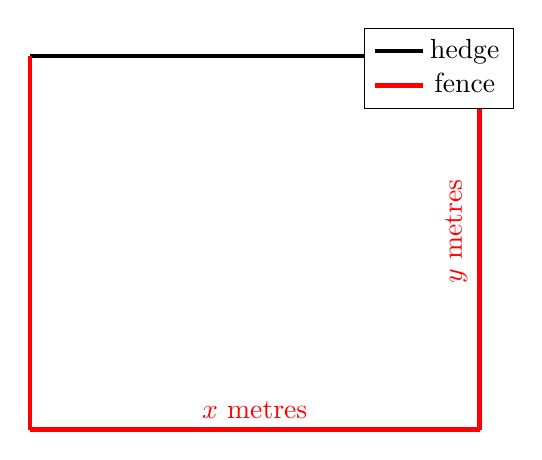
\begin{tikzpicture}
                    \begin{axis}[
                        axis lines = none,
                        ticks=none,
                    ]
                    \addplot [
                        domain=2:6, 
                        samples=100, 
                        color=black,
                        smooth,
                        ultra thick
                    ]
                    {4};
                    \addlegendentry{hedge}
                    \addplot [
                        domain=2:6, 
                        samples=100, 
                        color=red,
                        smooth,
                        ultra thick
                    ]
                    {2} node[above, pos=0.5] {$x$ metres};
                    \addplot +[mark=none, color=red, smooth, ultra thick] coordinates {(2, 2) (2, 4)};
                    \addplot +[mark=none, color=red, smooth, ultra thick] coordinates {(6, 2) (6, 4)} node[left, pos=0.7, xshift=-0.3cm, rotate=90] {$y$ metres};
                    \addlegendentry{fence}
                    \end{axis}
                \end{tikzpicture}\n
                Notice that from the diagram, the fence will take up 2 times of its height $y$ and its length $x$. Thus:
                \[\begin{split}
                    x + 2y &= 120\\
                    2y &= 120 - x\\
                    y &= \frac{1}{2}(120-x)
                \end{split}\] 
                And the area of the pen is:
                \[\begin{split}
                    A &= xy
                \end{split}\]
                Substitute $y$ with the expression we just derived:
                \[\begin{split}
                    A &= x\left(\frac{1}{2}(120-x)\right)\\
                    A &= \frac{1}{2}x(120-x)
                \end{split}\]
                And we finally arrive at the required expression for the area of the pen.\n
                \bd{(b)} To find the maximum area, we can look for the stationary point of the function $A$ by first differentiating:
                \[\begin{split}
                    A &= \frac{1}{2}x(120-x)\\
                    A &= 60x - \frac{1}{2}x^2\\
                    \frac{dA}{dx} &= 60 - x\\
                \end{split}\]
                Equate to zero:
                \[\begin{split}
                    0 &= 60-x\\
                    x &= 60
                \end{split}\]
                At $x=60$, the area of the sheep pen is:
                \[\begin{split}
                    A &= \frac{1}{2}x(120-x)\\
                    A &= \frac{1}{2}(60)(120-60)\\
                    A &= 1800
                \end{split}\]
                Obtaining $A = 1800m^2$ as the maximum possible area.
            
            \subsubsection{Problem 7}
                An open cylindrical wastepaper bin, of radius $r$ $cm$ and capacity $V$ $cm^3$, is to have a surface area of $5000 cm^2$.\n
                (a) Show that $V = \frac{1}{2}r(5000-\pi r^2)$.\n
                (b) Calculate the maximum possible capacity of the bin.\n
                \bd{Solution}\n
                \bd{(a)} Again, we need to find expressions that represents the quantities we are dealing with, namely \bd{volume} and \bd{surface area}.\n
                We know that the volume of a cylinder is given by:
                \begin{equation}
                    V = \pi r^2h
                \end{equation}
                and its surface area (of an \bd{open} cylinder):
                \begin{equation}
                    A = 2\pi r h + \pi r^2
                \end{equation}
                Since we do know that the surface area is $5000cm^2$, we can re-arrange expression $(3)$ with $h$ as the subject:
                \[\begin{split}
                    5000 &= 2\pi r h + \pi r^2\\
                    2\pi r h &= 5000 - \pi r^2 \\
                    h &= \frac{5000 - \pi r^2}{2\pi r}
                \end{split}\]
                Then, we can substitute $h$ in $(2)$ with the newly formed expression:
                \[\begin{split}
                    V &= \pi r^2h\\
                    V &= \pi r^2 \left(\frac{5000 - \pi r^2}{2\pi r}\right)\\
                    V &= r \left(\frac{5000 - \pi r^2}{2}\right)\\
                    V &= \frac{1}{2}r(5000 - \pi r^2)\\
                \end{split}\]
                Arriving at the required form.\n
                \bd{(b)} To find the maximum capacity (volume), we can find the stationary point of the function $V$ by differentiating it:
                \[\begin{split}
                    V &= \frac{1}{2}r(5000 - \pi r^2)\\
                    V &= 2500r - \frac{1}{2}\pi r^3\\
                    \frac{dV}{dr} &= 2500 - \frac{3}{2}\pi r^2
                \end{split}\]
                Equate to zero and solve for $r$:
                \[\begin{split}
                    0 &= 2500 - \frac{3}{2}\pi r^2\\
                    \frac{3}{2}\pi r^2 &= 2500\\
                    r^2 &= \frac{5000}{3\pi}\\
                    r &= \pm \sqrt{\frac{5000}{3\pi}}
                \end{split}\]
                Since radius $r$ can only be of positive value:
                \[r = \sqrt{\frac{5000}{3\pi}}\]
                And at $r = \sqrt{\frac{5000}{3\pi}}$, the volume of the bin:
                \[\begin{split}
                    V &= 2500r - \frac{1}{2}\pi r^3\\
                    V &= 2500\left(\sqrt{\frac{5000}{3\pi}}\right) - \frac{1}{2} \pi \left(\sqrt{\frac{5000}{3\pi}}\right)^3\\
                    V &\approx 38388
                \end{split}\]
                Therefore, the maximum possible capacity of the bin is approximately $38388cm^3$
    \bibliographystyle{apacite}
    \bibliography{References}

\end{document}